\documentclass[12pt,convert={false}]{standalone}
\usepackage[dvipsnames]{xcolor}
\usepackage{tikz}
\usetikzlibrary{shapes,arrows,positioning,calc,patterns,arrows.meta, bending, graphs, shadings,quotes,intersections}
\usetikzlibrary{external}
%\tikzexternalize[prefix=tikz/]
\usepackage{pgfplots}
\pgfplotsset{compat=1.16}
\usepgfplotslibrary{fillbetween}
\newcommand{\enf}[1]{\textcolor{RedViolet}{\textbf{#1}}} %enf sta per enfasi
\newcommand{\sott}[1]{\setulcolor{black!20!Goldenrod}\ul{#1}}
\newcommand{\prob}{\mathbb{P}}
\newcommand\independent{\protect\mathpalette{\protect\independenT}{\perp}}
\newcommand{\ev}[1]{\mathbb{E}\Bigl[{#1}\Bigr]}
\def\independenT#1#2{\mathrel{\rlap{$#1#2$}\mkern2mu{#1#2}}}
\newcommand{\Z}{\mathbb{Z}}
\newcommand{\R}{\mathbb{R}}
\newcommand{\N}{\mathbb{N}}
\newcommand{\equalexpl}[1]{%
	\underset{\substack{\uparrow\\\mathrlap{\text{\vspace{-3cm}\hspace{-1em}#1}}}}{=}}
\newcommand{\dif}{\mathop{}\!\mathrm{d}}
\begin{document}
    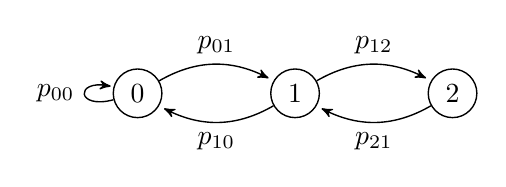
\begin{tikzpicture}[->,>=stealth',shorten >=2pt, line width=0.5pt, node distance=2cm]
	\node [circle, draw] (zero) {0};
	\node [circle, draw] (one) [right of=zero] {1};
	\node [circle, draw] (two) [right of=one]{2};
	\path (zero) edge [bend left] node [above] {$p_{01}$} (one);
	\path (one) edge [bend left] node [above] {$p_{12}$} (two);
	\path (zero) edge [loop left] node [left] {$p_{00}$} (zero);
	\path (two) edge [bend left] node [below] {$p_{21}$} (one);
	\path (one) edge [bend left] node [below] {$p_{10}$} (zero);
\end{tikzpicture}
\end{document}
